\documentclass[xcolor=table]{beamer}
\usetheme{Rochester}
\usepackage{amsmath}
\usepackage{amssymb}
\usepackage{graphicx}
\usepackage{tikz}
\usepackage{pgfplots}
\pgfplotsset{compat=1.18}
\usetikzlibrary{arrows.meta}
\usetikzlibrary{calc}
\usetikzlibrary{decorations.pathmorphing}
\newcommand*\circled[1]{\tikz[baseline=(char.base)]{
            \node[shape=circle,draw, minimum size=3.5mm,inner sep=0.5pt] (char) {#1};}}

\usepackage{ifthen}
\usepackage[noend]{algpseudocode}
\usepackage{soul}
\usepackage{isabelle}
\usepackage{isabellesym}
\isabellestyle{it}

\DeclareMathOperator{\mbind}{\text{\isa{\isasymbind}}}
\DeclareMathOperator{\expect}{\mathrm{E}}

\renewcommand{\algorithmicrequire}{\textbf{Input:}}
\renewcommand{\algorithmicensure}{\textbf{Output:}}
\newcommand{\ift}[3]{\mathbf{if} \; #1 \; \mathbf{then} \; #2 \; \mathbf{else} \; #3}
\newcommand{\integral}[3]{\int_{#1} \! #2 \, \mathrm{d} #3}

\newcommand{\getsr}{\xleftarrow{\$}}
\newcommand{\robot}[1]{\includegraphics[width=#1]{contrib/vecteezy_cute-robot-holding-clipboard-cartoon-icon-illustration_53779545_655/vecteezy_cute-robot-holding-clipboard-cartoon-icon-illustration_53779545}}

\title{Verification of the CVM algorithm with a Functional Probabilistic Invariant}
\author{E. Karayel\inst{1}, J. Watt\inst{2}, D. Khu\inst{2}, K. Meel\inst{4,5}, Y. K. Tan\inst{2,3}}
\institute[VFU]{
  \inst{1}%
    Technical University of Munich, Germany
  \and
  \inst{2}%
    Institute for Infocomm Research (I$^2$R), A*STAR, Singapore
  \and
  \inst{3}%
    Nanyang Technological University, Singapore
  \and
  \inst{4}%
    Georgia Institute of Technology, Atlanta, GA, USA
  \and
  \inst{5}%
    University of Toronto, Canada
}

\usepackage{mathtools}
\DeclareMathOperator{\prob}{\mathcal P}
\DeclareMathOperator{\bigo}{\mathcal O}
\DeclarePairedDelimiter{\ceil}{\lceil}{\rceil}
\DeclareMathOperator{\Ber}{\mathrm{Ber}}
\DeclareMathOperator{\indicat}{\mathrm{I}}

\begin{document}
\AtBeginSection[]
{
    \begin{frame}
        \frametitle{Table of Contents}
        \tableofcontents[currentsection]
    \end{frame}
}

\frame{\titlepage}
\begin{frame}
\frametitle{Table of Contents}
\tableofcontents
\end{frame}

\section{Introduction}
\label{sec:intro}

In 2022, Chakraborty, Vinodchandran, and Meel~\cite{chakraborty2022} published a marvelous streaming algorithm for the distinct elements problem which was very unexpected in the community~\cite{quanta}.
Indeed, Knuth later wrote a note on the algorithm~\cite{knuthnote}, pointing out its interesting properties and christening it the \emph{CVM} algorithm (which we use for the rest of this paper).
One striking property of the CVM algorithm is that, in contrast to every other known algorithm for the problem, it does not rely on hashing the stream elements.
Instead, the algorithm could theoretically be implemented in a setting where objects in the data stream only allow for equality comparisons.

Another property of CVM is its simplicity, both in terms of its description---the algorithm is listed in its entirety in~\cref{alg:cvm}---and its pen-and-paper correctness proof, which only requires undergraduate-level exposure to randomized algorithms.
This is why its authors called it ``an algorithm for the text book''.
The motivation of this work is to explore whether CVM's simplicity transfers into a mechanization within the Isabelle proof assistant~\cite{nipkow2002}.

\begin{algorithm}[h!]
	\caption{CVM algorithm for distinct elements estimation~\cite{chakraborty2022}.}\label{alg:cvm}
	\begin{algorithmic}[1]
  \Require Stream elements $a_1,\dots,a_l$, $0 < \varepsilon$, $0 < \delta < 1$.
  \Ensure A cardinality estimate $R$ for set $A = \{ a_1,\dots,a_l \}$ s.t. $\prob \left( |R - |A| | > \varepsilon |A| \right) \leq \delta$
  \State $\chi \gets \{\}, p \gets 1, n = \ceil*{\frac{12}{\varepsilon^2} \ln{(\frac{6l}{\delta})} }$
  \For{$i \gets 1$ to $l$}
    \State $b \getsr \Ber(p)$ \Comment insert $a_i$ with probability $p$ (and remove it otherwise)
    \If{$b$}
      \State $\chi \gets \chi \cup \{a_i\}$
    \Else
      \State $\chi \gets \chi - \{a_i\}$
    \EndIf
    \If{$|\chi| = n$}
      \State $\chi \getsr \mathrm{subsample}(\chi)$ \Comment discard elements of $\chi$ independently with prob. $\frac{1}{2}$
      \State $p \gets \frac{p}{2}$
    \EndIf
    \If{$|\chi| = n$}
      \Return $\bot$ \Comment fail if $\chi$ remains too large
    \EndIf
  \EndFor
  \State \Return $\frac{|\chi|}{p}$ \Comment estimate cardinality of $A$
  \end{algorithmic}
\end{algorithm}

Curiously, our formalization takes a substantially different route compared to the original proof~\cite{chakraborty2022,DBLP:journals/corr/abs-2301-10191}.
Briefly, the pen-and-paper analysis for CVM relies on a sequence of transformations of the algorithm.
The reason for these transformations is that standard methods for analyzing randomized algorithms, such as Chernoff--Hoeffding bounds, usually make statements about independent random variables.
Yet, for~\cref{alg:cvm} the random operations are far from being independent.\footnote{This was an incorrect claim in the initial published proof of CVM~\cite[Claim 6]{chakraborty2022}; a later version by the same authors~\cite{DBLP:journals/corr/abs-2301-10191} provides a correct proof.
The original error serves as a side motivation for this work.}
For example, in line 3 the Bernoulli distribution is sampled for a value $p$, which itself depends on previous random operations; similarly, the subsampling step in line 9 is only applied if the buffer is full, which also depends on previous random operations.
The aforementioned sequence of transformations bounds the error of~\cref{alg:cvm} in terms of another randomized algorithm with more desirable independence properties.
Indeed, it seems impossible to analyze~\cref{alg:cvm} directly using known methods.

This is the point where our new analysis technique comes in---it is very similar to how deterministic algorithms are verified using a loop invariant.
The key difference is that our choice of ``loop invariant'' for the randomized streaming algorithm is a functional probabilistic inequality, namely, we consider invariants of the form:
\[
  \expect [ h ] \leq h(c)
\]
where $h$ is allowed to range over a class of functions, and the expectation is taken over the distribution of the state of the algorithm after consuming each stream element.
By first establishing such an invariant for~\cref{alg:cvm}, we can then use it (via different choices of $h$) to establish error bounds for the algorithm.
For the rest of this paper, we explain this technique, its mechanization, and show how it leads to a simple but substantially more general proof of the CVM algorithm.
We believe the new proof remains accessible at the undergraduate level, albeit with some exposure to interactive theorem proving.

The main contributions of this work are:
\begin{itemize}
\item Introduction of a new technique using functional probabilistic invariants to verify randomized algorithms inductively/recursively.
\item Verification of the original CVM algorithm using our new technique.
\item Presentation and verification of a new variant of CVM that is total and unbiased.
\item Formalization of a theory of negatively associated random variables used to analyze the new CVM variant.
\end{itemize}

Verification of CVM using our new technique requires only 1044 lines in Isabelle~\cite{nipkow2002}, while the original proof required \todo{x} lines.
We detail some of the challenges faced when mechanizing the reduction arguments used by Chakraborty et al.~\cite{chakraborty2022,DBLP:journals/corr/abs-2301-10191} in Section~\todo{x}.

The formalized CVM variant showcases the utility of our new proof technique.
In this variant, the subsampling step in line 9 of \cref{alg:cvm} selects a random $m$-sized subset of $\chi$, instead of independently deciding for each element, whether to keep it.
This variant has the benefit that it is \emph{total} (never returns $\bot$) because the second check in line 11 becomes obsolete.
More interestingly, the resulting variant is \emph{unbiased}, i.e., the expected result is exactly the cardinality of the elements in the stream; this is a new property, that neither the original CVM algorithm nor classic algorithms for the distinct elements problem possess.

To analyze the new variant, we use results from the theory of negatively dependent random variables to establish the desired functional invariant.
The concept of negative association is a generalization of independence; negatively associated variables observe closure properties and fulfill Chernoff--Hoeffding bounds similar to independent random variables.
It should be stressed that the theory of negatively associated RVs is orthogonal to our new technique, but the formalization of such a theory is also a contribution of this work.

% TODO: move it into the discussion of the variant, I think it is better once the algorithm is shown
%This is because indicator functions of $n$-subsets form negatively associated random variables (RV), even though they are not independent, with which we can modify the subsampling step to the form we described above.

% TODO: move it into explanation of the technique
%Note that we are able to establish tail bounds using these invariants, which has, so far, not been possible using a simple loop invariant for randomized algorithms.
%The loop invariants are established, essentially, using the key property of the Giry monad:
%\[
%  \expect_{m \isa{\isasymbind} f} [h] = \int_m \expect_{f (x)} [h] \, d x \textrm{.}
%\]
%Here $m \isa{\isasymbind} f$ denotes distribution of a randomized algorithm, which represents the sequential composition of $m$ with $f$.

%TODO: I think this should be later, we can give a forward reference
%% The algorithm's state is a buffer $\chi$  (initially empty) and a fraction $p > 0$ (initially set to $1$).
%% The buffer contains a subset of the elements of the stream encountered so far, with maximal size $n$.
%% The size is chosen according to the desired accuracy parameters $\varepsilon$, $\delta$, and the stream size $l$.
%% The algorithm iterates over stream elements, adding each one to the buffer with probability $p$ or conversely -- if the current stream element is already in the buffer -- removing them with probability $(1-p)$.
%% If the buffer gets too large, approximately half of the elements are removed by discarding each element in $\chi$ independently with probability $\frac{1}{2}$; then, $p$ is adjusted to reflect the fact that the buffer now contains each element with probability $p_\text{new} = \frac{p_\text{old}}{2}$.
%% After processing the stream, the algorithm returns $\frac{|\chi|}{p}$ as an approximation of the number of distinct elements in the stream.
%% This output is probably-approximately correct, i.e., the probability that the relative error of $\frac{|\chi|}{p}$ exceeds $\varepsilon$ is at most $\delta$.
%The output of CVM is \emph{probably-approximately correct}, i.e., the probability that the relative error of its output exceeds $\varepsilon$ is at most $\delta$.
%Moreover, let us assume the space needed to store each element in the stream is $b$ bits, then the algorithm requires only $\bigo(\varepsilon^{-2} b \ln(\delta^{-1} l))$ bits of mutable state---far less than storing each stream element deterministically.%
%\footnote{The optimal randomized algorithm requires $\bigo( \varepsilon^{-2} \ln \delta + b)$ bits, but it requires more advanced algorithmic techniques. It would not be possible to present using such elementary steps as used in \cref{alg:cvm}, and involves computations in finite fields and random walks in expander graphs~\cite{blasiok2020, karayel2023}.}
%

\todo{Classic summary of sections.}


%% We set out to formalize the proof as described in the literature~\cite{chakraborty2022}, hoping to show that it would also be an easy formalization exercise.

%% %TODO: a bit too long in details, we should trim this and move to later section
%% \subparagraph*{The road not taken:}
%% One of the difficult aspects of the proof is that it relies on an eager-lazy coin flip conversion.
%% To understand that, we should note that none of the observable random variables, such as the presence of a stream element in the buffer or conditions on the value of $p$, are independent of the other state variables, which makes the algorithm hard to analyze and makes the application of standard techniques from probability theory, such as Hoeffding's theorem impossible.
%% The authors resolved that problem by a simulation argument---they show that~\cref{alg:cvm} behaves stochastically identically to a different algorithm, which makes the relevant coin flips in a different order.
%% That modified algorithm performs a column of coin flips for each stream element.
%% An element is kept in the buffer if the first $k=\log_2(p-1)$ rows of the column are heads.
%% At each sub-sampling step, when p is divided by two, i.e., if k increases by one.
%% The algorithm examines the newly activated $k$-th row of the previous sequence elements to decide whether the element should be kept in the buffer.
%% This preserves the invariant that the buffer consists of exactly those sequence elements whose associated coin flip column starts with $\log_2(p-1)$ heads.
%% Of course, the new algorithm is not practical for actual implementation, but one can verify its correctness using standard Chernoff bounds, and on the other hand, it is possible to show that its behavior is equivalent to Algorithm 1.
%% To summarize, while the algorithm is marvelous, the proof was still very technical.
%% The simulation argument, in particular, is not so elegant to formalize.

%% \subparagraph*{A more direct proof:}
%% We set out to try to find a more direct proof, which also eases the formalization effort.
%% For the following discussion, we will analyze Algorithm 1 with line 8 removed, i.e., the algorithm does not output $\bot$, nor performs a second check of $|\chi|=n$.
%% Note that this happens if the very improbable event where none of the elements in X are removed during a subsampling step, which happens with probability at most $2^{-n/2}$.
%% Overall, the probability of it happening during the course of the algorithm is at most $\frac{\delta}{2}$. (Note that removing line 8 does not affect the correctness of the algorithm, but it loses its space consumption bound.)
%% It is easy to see that any probability established about the algorithm missing line 8 will be true for the original algorithm with a possible correction by, at most,  $\frac{\delta}{2}$.
%% We will remember and correct this at the end of this section.

%% Let us consider an imaginary situation where, somehow, $p$ is fixed at some point in the algorithm.
%% For example, we could imagine a final sub-sampling loop, which is run until a fixed $p$ is reached.
%% Then, the indicator random variables representing the presence of a stream element TODO


\section{Verification using Functional Probabilistic Invariants}
\begin{frame}<1-5>[label=algsplit]
\frametitle{Another slide with the algorithm}
\begin{algorithmic}
  \State $\chi \gets \{\}, p \gets 1, n = \ceil*{\frac{12}{\varepsilon^2} \ln{(\frac{\only<6>{3}\only<1-5>{6}l}{\delta})} }$
  \For{$i \gets 1$ to $l$}
    \State $b \getsr \Ber(p)$
    \If{$b$}
      \State $\chi \gets \chi \cup \{a_i\}$
    \Else
      \State $\chi \gets \chi - \{a_i\}$
    \EndIf
    \If{$|\chi| = n$}
      \State $\chi \getsr \only<1-5>{\mathrm{subsample}}\only<6>{\mathrm{subsample'}}(\chi)$
      \State $p \gets \frac{p}{2}$
    \EndIf
    \If{$|\chi| = n$}
      \Return $\bot$
    \EndIf
  \EndFor
  \State \Return $\frac{|\chi|}{p}$
\end{algorithmic}

\tikz[overlay, shift=(current page.north west)]{
\begin{scope}[x={(current page.north east)},y={(current page.south west)}]

\only<2->{
        \fill[blue!50, opacity=0.5] (0.07,0.4) rectangle (0.7,0.67);
        \node [anchor=west] at (0.45,0.535) {Step 1};
}
\only<3->{
        \fill[red!50, opacity=0.5] (0.07,0.675) rectangle (0.7,0.845);
        \node [anchor=west] at (0.45,0.76) {Step 2};
}
\only<4->{
        \draw[thick, decorate, decoration={snake,amplitude=0.6pt}] (0.072,0.87) -- (0.42, 0.87);
}
\only<6>{
       \fill[white] (0.07,0.846) rectangle (0.7,0.895);
}
\only<5->{
  \fill[green!50, opacity=0.5] (0.03, 0.895) rectangle (0.7, 0.97);
   \node [anchor=west] at (0.45,0.932) {Estimate};
}
\end{scope}
}
\end{frame}

\begin{frame}
\frametitle{Giry Monad}
We can represent randomized algorithms using the Giry monad:
\begin{itemize}
\item Primitive random operations, e.g., $\Ber(p)$
\item Return operation $\mathrm{return} \, x$
\item Sequential compositon $m \mbind f$
\end{itemize}
\pause
\begin{block}{Fact}
For an event $E$: 
\begin{eqnarray*}
\prob_{m \mbind f}( E )  & = & \int_{m} P_{f(x)} (E) \, dx \onslide<3->{= \sum_x P_{f(x)} (E) P_m({x})} \\
\onslide<4->{\expect_{m \mbind f}[ g ]  & = & \int_{m} \expect_{f(x)} [g] \, dx}
\end{eqnarray*}
\end{block}
\end{frame}

\againframe<5>{algsplit}

\begin{frame}
\frametitle{Our algorithm in monadic notation}
\newcommand{\stepone}{\textcolor{blue}{\mathrm{step}_1}}
\newcommand{\steptwo}{\textcolor{red}{\mathrm{step}_2}}
\newcommand{\estimate}{\textcolor{green}{\mathrm{estimate}}}
\begin{eqnarray*}
  \mathrm{init} & \mbind & \stepone a_1 \mbind \steptwo \mbind \stepone a_2 \mbind \steptwo \cdots \\
  & \mbind & \stepone a_l \mbind \steptwo \mbind \estimate \\
  \mathrm{init} & = & \mathrm{return} \, (1, \emptyset)
\end{eqnarray*}
\pause
Example invariant:
\[
\expect \left[ \frac{\indicat(s \in \chi)}{p} \right]= 1
\]
for all $s$ that are present in the stream.
\end{frame}

\begin{frame}
\frametitle{Verifying the invariant: Induction step for Step 2}
\begin{block}{Assumption}
$\expect_m \left[ \frac{\indicat(s \in \chi)}{p} \right] = 1$
\end{block}
\begin{block}{Goal}
$ L := \expect_{m \mbind \mathrm{step}_2} \left[ \frac{\indicat(s \in \chi)}{p} \right]= 1$
\end{block}
\[
L =
\only<1>{\expect_{m \mbind \mathrm{step}_2} \left[ \frac{\indicat(s \in \chi)}{p} \right]}
\only<2>{\integral{m}
      {\left(\ift{|\chi|=n}{\integral{\mathrm{subs.}(\chi)}{\frac{\indicat(s \in \tau)}{p/2}}{\tau}}{\frac{\indicat(s \in \chi)}{p}} \right)}
      {\sigma}}
\only<3>{\integral{m}
      {\left(\ift{|\chi|=n}{\frac{2}{p}\integral{\mathrm{subs.}(\chi)}{\indicat(s \in \tau)}{\tau}}{\frac{\indicat(s \in \chi)}{p}} \right)}
      {\sigma}}
\only<4>{\integral{m}
      {\left(\ift{|\chi|=n}{\frac{2}{p}\frac{\indicat(s \in \chi)}{2}}{\frac{\indicat(s \in \chi)}{p}} \right)}
      {\sigma}}
\only<5>{\integral{m}
      {\left(\ift{|\chi|=n}{\frac{\indicat(s \in \chi)}{p}}{\frac{\indicat(s \in \chi)}{p}} \right)}
      {\sigma}}
\only<6>{\integral{m}
      {\frac{\indicat(s \in \chi)}{p} }
      {\sigma}}
\only<7>{1}
\]
\end{frame}

\begin{frame}[label=observations]
\frametitle{Observations}
\begin{itemize}
\item Expected result is the count of distinct elements.
\only<2->{\item We want to establish concentration}
\only<4->{\item Can extend the above recursive analysis to more complex expressions: }
\only<5>{
\[
  \expect \left[ h \left( \frac{\indicat(s \in \chi)}{p} \right)\right] \leq h(1)
\]
for every non-negative concave function $h$ and stream elements $s$.}
\only<6->{
\[
  \expect \left[ \prod_{s \in S}  h \left( \frac{\indicat(s \in \chi)}{p} \right)\right] \leq h(1)^{|S|}
\]
for every non-negative concave function $h$ and subset of stream elements $S$.}
\only<7->{\item $\Rightarrow$\only<8->{*} Approximation Guarantee
\[
  \prob\left(|X - |A|| \geq \varepsilon |A| \right) \leq \delta 
\]
\only<8->{\item More details in the paper.}
}
\end{itemize}
\only<3>{
\begin{figure}
\centering
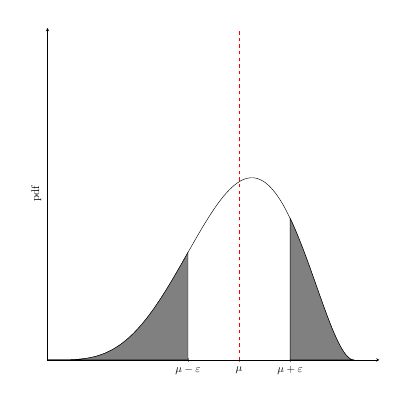
\begin{tikzpicture}[scale=0.4]
\begin{axis}[
    xmin=0, xmax = 6.5,
    ymin=0, ymax=0.7,
    axis lines = left,
    xlabel = {},
    xtick={2.75,3.75,4.75},
    xticklabels={$\mu-\varepsilon$,$\mu$,$\mu+\varepsilon$},
    ytick=\empty,
    ylabel = {pdf},
    height = \textwidth,
    width = \textwidth,
]
\addplot [
    domain=0:6, 
    samples=1000, 
]{max(0,35/2*(x/6)^4*(1-x/6)^2)};
\addplot [
    domain=4.75:6, 
    samples=1000, 
    fill=gray,
]{max(0,35/2*(x/6)^4*(1-x/6)^2)} \closedcycle;
\addplot [
    domain=0:2.75, 
    samples=1000, 
    fill=gray,
]{max(0,35/2*(x/6)^4*(1-x/6)^2)} \closedcycle;
\draw[color=red, dashed] (axis cs:3.75, 0) -- (axis cs:3.75, 0.7);
\end{axis}
\end{tikzpicture}
\begin{tikzpicture}[scale=0.4]
\begin{axis}[
    xmin=0, xmax = 6.5,
    ymin=0, ymax=0.7,
    axis lines = left,
    xlabel = {},
    xtick={2.75,3.75,4.75},
    xticklabels={$\mu-\varepsilon$,$\mu$,$\mu+\varepsilon$},
    ytick=\empty,
    ylabel = {pdf},
    height = \textwidth,
    width = \textwidth,
]
\addplot [
    domain=0:6, 
    samples=1000, 
]{0.65*exp(-(2*(x-3.75))^2)};
\addplot [
    domain=4.75:6, 
    samples=1000, 
    fill=gray,
]{0.65*exp(-(2*(x-3.75))^2)} \closedcycle;
\addplot [
    domain=0:2.75, 
    samples=1000, 
    fill=gray,
]{0.65*exp(-(2*(x-3.75))^2)} \closedcycle;
\draw[color=red, dashed] (axis cs:3.75, 0) -- (axis cs:3.75, 0.7);
\end{axis}
\end{tikzpicture}
\end{figure}
}
\end{frame}

\begin{frame}
\frametitle{Observations II}
\begin{itemize}
\item The new proof is much shorter than the original proof (1003 lines vs. 2634 lines.)
\item<2-> \emph{As far as we can tell,} this technique is new.
\item<3-> The new proof opens up the design-space of the algorithm.
\item<4,6-> \only<4>{For example we can select the subsampling ratio dynamically.}\only<6->{More interestingly: It is possible to use a different subsampling operation.}
\item<7-> Select a random $nf$-subset (where $\frac{1}{2} \leq f < 1$, $nf \in \mathbb Z$).
\item<8-> $\Rightarrow$ Unbiased algorithm
\end{itemize}
\end{frame}
\againframe<5-6>{algsplit}



\section{Original Proof}
In this section we describe the interesting parts of the original proof by Chakraborty et al.~\cite{chakraborty2022}.
This highlights in part, why it requires a lot of work to formalize, and why we were motivated to develop our new approach using probabilistic invariants.

As we mentioned in the introduction, the main difficulty is the fact that \cref{alg:cvm}'s state variables are not independent.
The trick Chakraborty et al. use to circumvent the problem is by modifying the algorithm, in a manner that obviously preserves its distribution, such that the resulting algorithm's state can be described in terms of independent coin flips.

Let us consider a state, where $k$ subsampling steps have been performed, i.e., $p = 2^{-k}$. 
Then the algorithm would normally perform a coin flip with probability $p$.
In the modified algorithm, we perform a fixed number of coin flips for each sequence element at the beginning.
The element is put into the sample, whenever the first $k$ coin flips associated with the sequence element are $1$.
Note that this happens exactly with probability $2^{-k}$, which means the behaviour of the algorithm is unchanged.

Moreover, during the subsampling operation those elements are kept, whose $k+1$-th associated coin flip is $1$.
This again preserves the behaviour, that each element is discared independently with probability $1/2$.
The operation $p \mapsto \frac{p}{2}$ is replaced with $k \mapsto k+1$.
For this modified algorithm, it is easy to see that the set of elements in any state are exactly, those stream elements for which the first $k$ entries of their associated coin flips are $1$.

In \cref{alg:cvm_simul} we describe the new algorithm, that behaves exactly as the original one (\cref{alg:cvm}), but performs indepenent coin flips.
Note that the function $\mathrm{last{\textunderscore}index}$ returns the index of the last-occurence of an element in the sequence, before the current loop iteration.
It should be noted that the algorithm keeps track of the number of subsampling iterations $k$, instead of the value $p = 2^{-k}$ as the original algorithm does.
%Like, we did in \cref{sec:invariants}, we ignore the second check, whether the subsampling operation succeeded.
%As we explained there, the total variational difference between these two variants is $\frac{\delta}{2}$.
%
\begin{algorithm}[h!]
	\caption{Modified CVM algorithm with independent coin flips.}\label{alg:cvm_simul}
	\begin{algorithmic}[1]
  \Require Stream elements $a_1,\dots,a_l$, $0 < \varepsilon$, $0 < \delta < 1$.
  \State $\chi \gets \{\}, k \gets 0, n = \ceil*{\frac{12}{\varepsilon^2} \ln{(\frac{6l}{\delta})} }$
  \State $b[i,j] \getsr \Ber(1/2)$ for $i,j \in \{1,\cdots,l\}$ \Comment perform $l^2$ unbiased independent coin flips
  \For{$i \gets 1$ to $l$}
    \If{$b[i,1]=b[i,2]=\cdots=b[i,k]=1$}
      \State $\chi \gets \chi \cup \{a_i\}$
    \Else
      \State $\chi \gets \chi - \{a_i\}$
    \EndIf
    \If{$|\chi| = n$}
      \State $\chi \gets \{a \in \chi | b[\mathrm{last{\textunderscore}index}(a),k+1] = 1\}$
      \State $k \gets k+1$
    \EndIf
    \If{$|\chi| = n$}
      \State \Return $\bot$
    \EndIf
  \EndFor
  \State \Return $2^k |\chi|$ \Comment estimate cardinality of $A$
  \end{algorithmic}
\end{algorithm}
To roughly explain, how tail bounds can be derived for this new variant:
It is possible to union bound the probability that the estimate exceeds the desired interval, with the probability of the event in conjunction with a specific value of $k$, which can be bounded by the probability that the number of stream elements with whose associated coin flips start with $k$ ones, is outside of $2^{-k} |A| (1 \pm \varepsilon)$.
This is explained in more detail by Chakraborty et al.~\cite{chakraborty2022}.

One of the key questions is, how to formalize the transformation from \cref{alg:cvm} to this new variant.
What we discovered is that it best to solve the problem backwards, i.e., we start with the modified algorithm, which performs all the coin-flips in advance --- eagerly --- and convert it to the version, that performs the coin flips --- lazily --- at the point they are needed.

We can push down the coin flips through the expression tree.
To explain how this works.
Let us first define the \emph{sampling} function, i.e., let $f$ be a function that depends on coin flips, more precisely $f$ takes as argument a vector of coin flips indexed by $I$, then we can express the distribution of $f$ with respect to indepenent unbiased coin flips as.
\begin{isabelle_cm}
  sample\ f\ \isacharequal\ map{\isacharunderscore}pmf\ f\ {\isacharparenleft}prod{\isacharunderscore}pmf\ I\ {\isacharparenleft}\isasymlambda\isacharunderscore\isachardot\ bernoulli{\isacharunderscore}pmf \isacharparenleft\isadigit{1}/\isadigit{2}\isacharparenright\isacharparenright\isacharparenright
\end{isabelle_cm}
%For example, we could use our modified algorithm as $f$, with the index set $I = \{0, \ldots, l-1\} \times \{0, \ldots, l-1\}$.
The interesting fact is that we can distribute the sampling operation over composition, e.g.:
\begin{isabelle_cm}
  sample\ \isacharparenleft\isasymlambda\isasymomega\isachardot\ f\ \isasymomega\ \isasymcirc\ g\ \isasymomega{\isacharparenright}\ \isacharequal\ sample\ g\ \isasymbind\ \isacharparenleft{\isasymlambda}x\isachardot\ sample\ \isacharparenleft\isasymlambda\isasymomega\isachardot\ f\ \isasymomega\isachardot\ x\isacharparenright\isacharparenright
\end{isabelle_cm}
if $f$ and $g$ depend on disjoint subsets of the coin flips.




\todo{Explain how we formalized the original proof by Chakraborty et al. + brief section on the lazify}  



\section{Conclusion}\label{sec:conclusion}
We presented the first formalization of the CVM algorithm using Isabelle/HOL.
Central to our formalization is a novel invariant-based proof technique for randomized algorithms which is inspired by our alternative analysis of the CVM algorithm via the Cram\'{e}r--Chernoff method.
Interestingly, the technique readily generalized to a new CVM variant with stronger properties (totality and unbiasedness)---we formalized this latter version using the same invariant, together with a new library of results for negative association.
In future work, it would be interesting to formalize other variations of subsampling for CVM.
More generally, one could further explore whether the technique we introduced here could be applied towards proofs of other randomized (streaming) algorithms.


\end{document}
